\method consistently outperforms state-of-the-art forecasting methods by large margins across multiple benchmarks and settings, especially in few-shot and zero-shot scenarios. We compared our approach against a broad collection of up-to-date models, including a recent study that fine-tunes language model for time series analysis~\citep{zhou2023one}. To ensure a fair comparison, we adhere to the experimental configurations in \citep{wu2022timesnet} across all baselines with a unified evaluation pipeline\footnote{https://github.com/thuml/Time-Series-Library}. We use Llama-7B~\citep{touvron2023llama} as the default backbone unless stated otherwise.

\noindent\textbf{Baselines.}
We compare with the SOTA time series models, and we cite their performance from \citep{zhou2023one} if applicable. Our baselines include a series of Transformer-based methods: PatchTST~\citeyearpar{nie2022time}, ESTformer~\citeyearpar{woo2022etsformer}, Non-Stationary Transformer~\citeyearpar{liu2022non}, FEDformer~\citeyearpar{zhou2022fedformer}, Autoformer~\citeyearpar{wu2021autoformer}, Informer~\citeyearpar{zhou2021informer}, and Reformer~\citeyearpar{kitaev2020reformer}. We also select a set of recent competitive models, including GPT4TS~\citeyearpar{zhou2023one}, \revision{LLMTime~\citeyearpar{gruver2023large},} DLinear~\citeyearpar{zeng2023transformers}, TimesNet~\citeyearpar{wu2022timesnet}, and LightTS~\citeyearpar{zhang2022less}. In short-term forecasting, we further compare our model with N-HiTS~\citeyearpar{challu2023nhits} and N-BEATS~\citeyearpar{oreshkin2019n}. More details are in \shortautoref{appx:related_work}.

\vspace{-2mm}
\subsection{Long-term Forecasting} \label{sec:long-term-forecasting}
\vspace{-2mm}

\noindent\textbf{Setups.} 
\revision{We evaluate on ETTh1, ETTh2, ETTm1, ETTm2, Weather, Electricity (ECL), Traffic, and ILI, which have been extensively adopted for benchmarking long-term forecasting models~\citep{wu2022timesnet}.}
Details of the implementation and datasets can be found in \shortautoref{appx:experiment_details}. The input time series length $T$ is set as 512, and we use four different prediction horizons $H \in \{96, 192, 336, 720\}$. The evaluation metrics include mean square error (MSE) and mean absolute error (MAE).

\noindent\textbf{Results.} 
\revision{Our brief results are shown in \shortautoref{tab:long-term-forecasting}}, where \method outperforms all baselines in most cases and significantly so to the majority of them. The comparison with GPT4TS~\citep{zhou2023one} is particularly noteworthy. GPT4TS is a very recent work that involves fine-tuning on the backbone language model. We note average performance gains of \revision{\textbf{12\%} and \textbf{20\%}} over GPT4TS and TimesNet, respectively. When compared with the SOTA task-specific Transformer model PatchTST, by reprogramming the smallest Llama, \method realizes an average MSE reduction of \revision{1.4\%}. Relative to the other models, e.g., DLinear, our improvements are also pronounced, exceeding \revision{\textbf{12\%}}.

\begin{table}[h]
\renewcommand\arraystretch{1.2}
\captionsetup{font=small} 
\caption{\revision{Long-term forecasting results. 
All results are averaged from four different forecasting horizons:  $H \in \{24, 36, 48, 60\}$ for ILI and  $\{96, 192, 336, 720\}$ for the others. A lower value indicates better performance. {\boldres{Red}}: the best, \secondres{Blue}: the second best. Our full results are in \shortautoref{appx:short-term}.}}
\label{tab:long-term-forecasting}
\vspace{-3mm}
\begin{center}
\begin{small}
\scalebox{0.60}{
\setlength\tabcolsep{3pt}
\begin{tabular}{c|cc|cc|cc|cc|cc|cc|cc|cc|cc|cc|cc|cc}
\toprule

\multicolumn{1}{c|}{\multirow{2}{*}{Methods}}
&\multicolumn{2}{c|}{\method{}} &\multicolumn{2}{c|}{GPT4TS} &\multicolumn{2}{c|}{DLinear} &\multicolumn{2}{c|}{PatchTST} &\multicolumn{2}{c|}{TimesNet }&\multicolumn{2}{c|}{FEDformer} &\multicolumn{2}{c|}{Autoformer} &\multicolumn{2}{c|}{Stationary} &\multicolumn{2}{c|}{ETSformer} &\multicolumn{2}{c|}{LightTS} &\multicolumn{2}{c|}{Informer} &\multicolumn{2}{c}{Reformer} \\

\multicolumn{1}{c|}{} & \multicolumn{2}{c}{\scalebox{0.99}{(\textbf{Ours})}} & 
\multicolumn{2}{|c|}{\scalebox{0.99}{\citeyearpar{zhou2023one}}} &
\multicolumn{2}{c|}{\scalebox{0.99}{\citeyearpar{zeng2023transformers}}} &
\multicolumn{2}{c|}{\scalebox{0.99}{\citeyearpar{nie2022time}}} & \multicolumn{2}{c|}{\scalebox{0.99}{\citeyearpar{wu2022timesnet}}} & \multicolumn{2}{c|}{\scalebox{0.99}{\citeyearpar{zhou2022fedformer}}} & \multicolumn{2}{c|}{\scalebox{0.99}{\citeyearpar{wu2021autoformer}}} & \multicolumn{2}{c|}{\scalebox{0.99}{\citeyearpar{liu2022non}}} &  \multicolumn{2}{c|}{\scalebox{0.99}{\citeyearpar{woo2022etsformer}}} & \multicolumn{2}{c|}{\scalebox{0.99}{\citeyearpar{zhang2022less}}}  & \multicolumn{2}{c|}{\scalebox{0.99}{\citeyearpar{zhou2021informer}}} & \multicolumn{2}{c}{\scalebox{0.99}{\citeyearpar{kitaev2020reformer}}}  \\

\midrule

\multicolumn{1}{c|}{Metric} & MSE  & MAE & MSE & MAE& MSE & MAE& MSE  & MAE& MSE  & MAE& MSE  & MAE& MSE  & MAE& MSE  & MAE& MSE  & MAE& MSE  & MAE& MSE  & MAE& MSE  & MAE\\
\midrule

\multirow{1}{*}{\rotatebox{0}{$ETTh1$}}
&\boldres{0.408} &\boldres{0.423} &0.465&0.455&0.422&0.437&\secondres{0.413}&\secondres{0.430}&0.458&0.450&0.440&0.460&0.496&0.487&0.570&0.537&0.542&0.510&0.491&0.479&1.040&0.795&1.029&0.805\\
\midrule

\multirow{1}{*}{\rotatebox{0}{$ETTh2$}}
&\secondres{0.334}&\secondres{0.383}&0.381&0.412&0.431&0.446&\boldres{0.330}&\boldres{0.379}&0.414&0.427&0.437&0.449&0.450&0.459&0.526&0.516&0.439&0.452&0.602&0.543&4.431&1.729&6.736&2.191\\
\midrule

\multirow{1}{*}{\rotatebox{0}{$ETTm1$}}
&\boldres{0.329}&\boldres{0.372}&0.388&0.403&0.357&\secondres{0.378}&\secondres{0.351}&0.380&0.400&0.406&0.448&0.452&0.588&0.517&0.481&0.456&0.429&0.425&0.435&0.437&0.961&0.734&0.799&0.671 \\
\midrule

\multirow{1}{*}{\rotatebox{0}{$ETTm2$}}
&\boldres{0.251}&\boldres{0.313}&0.284&0.339&0.267&0.333&\secondres{0.255}&\secondres{0.315}&0.291&0.333&0.305&0.349&0.327&0.371&0.306&0.347&0.293&0.342&0.409&0.436&1.410&0.810&1.479&0.915 \\
\midrule

\multirow{1}{*}{\rotatebox{0}{\revision{$Weather$}}}
&\boldres{0.225} &\boldres{0.257} &0.237 &0.270 &0.248 &0.300 &\boldres{0.225} &\secondres{0.264} &0.259 &0.287 &0.309 &0.360 &0.338 &0.382 &0.288 &0.314 &0.271 &0.334 &0.261 &0.312 &0.634 &0.548 &0.803 &0.656 \\
\midrule

\multirow{1}{*}{\rotatebox{0}{\revision{$ECL$}}}
&\boldres{0.158} &\boldres{0.252} &0.167 &0.263 &0.166 &0.263 &\secondres{0.161} &\boldres{0.252} &0.192 &0.295 &0.214 &0.327 &0.227 &0.338 &0.193 &0.296 &0.208 &0.323 &0.229 &0.329 &0.311 &0.397 &0.338 &0.422 \\
\midrule

\multirow{1}{*}{\rotatebox{0}{\revision{$Traffic$}}}
&\boldres{0.388} &\secondres{0.264} &0.414 &0.294 &0.433 &0.295 &\secondres{0.390} &\boldres{0.263} &0.620 &0.336 &0.610 &0.376 &0.628 &0.379 &0.624 &0.340 &0.621 &0.396 &0.622 &0.392 &0.764 &0.416 &0.741 &0.422 \\
\midrule

\multirow{1}{*}{\rotatebox{0}{\revision{$ILI$}}}
&\boldres{1.435} &\secondres{0.801} &1.925 &0.903 &2.169 &1.041 &\secondres{1.443} &\boldres{0.797} &2.139 &0.931 &2.847 &1.144 &3.006 &1.161 &2.077 &0.914 &2.497 &1.004 &7.382 &2.003 &5.137 &1.544 &4.724 &1.445 \\
\midrule

\multicolumn{1}{c|}{$1^{\text{st}}$Count}&\multicolumn{2}{c|}{\boldres{7}}&\multicolumn{2}{c|}{0}&\multicolumn{2}{c|}{0}&\multicolumn{2}{c|}{\secondres{5}}&\multicolumn{2}{c|}{0}&\multicolumn{2}{c|}{0}&\multicolumn{2}{c|}{0}&\multicolumn{2}{c|}{0}&\multicolumn{2}{c|}{0}&\multicolumn{2}{c|}{0}&\multicolumn{2}{c|}{0}&\multicolumn{2}{c}{0}\\

\bottomrule
\end{tabular}
}
\end{small}
\end{center}
\end{table}

\subsection{Short-term Forecasting}
\vspace{-2mm}
\begin{table}[h]
\renewcommand\arraystretch{1.2}
% \vskip -0.15in
\captionsetup{font=small} 
\caption{Short-term time series forecasting results on M4. The forecasting horizons are in [6, 48] and the three rows provided are weighted averaged from all datasets under different sampling intervals. A lower value indicates better performance. \boldres{Red}: the best, \secondres{Blue}: the second best. 
\revision{More results are in \shortautoref{appx:short-term}.}
}
\label{tab:short-term-forecasting-brief}
\vspace{-4mm}
\begin{center}
\begin{small}
\scalebox{0.65}{
\setlength\tabcolsep{2.5pt}
\begin{tabular}{cc|cccccccccccccc}
\toprule

\multicolumn{2}{c|}{\multirow{2}{*}{Methods}}
& \multicolumn{1}{c|}{\method{}} &\multicolumn{1}{c|}{GPT4TS}&\multicolumn{1}{c|}{TimesNet}&\multicolumn{1}{c|}{PatchTST}&\multicolumn{1}{c|}{N-HiTS}&\multicolumn{1}{c|}{N-BEATS}& \multicolumn{1}{c|}{ETSformer}& \multicolumn{1}{c|}{LightTS}& \multicolumn{1}{c|}{DLinear} &\multicolumn{1}{c|}{FEDformer} &\multicolumn{1}{c|}{Stationary} &\multicolumn{1}{c|}{Autoformer}  &\multicolumn{1}{c|}{Informer} &\multicolumn{1}{c}{Reformer} \\

\multicolumn{2}{c|}{} & \multicolumn{1}{c}{\scalebox{0.99}{(\textbf{Ours})}} & 
\multicolumn{1}{|c|}{\scalebox{0.99}{\citeyearpar{zhou2023one}}} &
\multicolumn{1}{c|}{\scalebox{0.99}{\citeyearpar{wu2022timesnet}}} &
\multicolumn{1}{c|}{\scalebox{0.99}{\citeyearpar{nie2022time}}} &
\multicolumn{1}{c|}{\scalebox{0.99}{\citeyearpar{challu2023nhits}}} &
\multicolumn{1}{c|}{\scalebox{0.99}{\citeyearpar{oreshkin2019n}}} &
\multicolumn{1}{c|}{\scalebox{0.99}{\citeyearpar{woo2022etsformer}}} &
\multicolumn{1}{c|}{\scalebox{0.99}{\citeyearpar{zhang2022less}}} &
\multicolumn{1}{c|}{\scalebox{0.99}{\citeyearpar{zeng2023transformers}}} &
\multicolumn{1}{c|}{\scalebox{0.99}{\citeyearpar{zhou2022fedformer}}} &
\multicolumn{1}{c|}{\scalebox{0.99}{\citeyearpar{liu2022non}}} &
\multicolumn{1}{c|}{\scalebox{0.99}{\citeyearpar{wu2021autoformer}}} &
\multicolumn{1}{c|}{\scalebox{0.99}{\citeyearpar{zhou2021informer}}} &
\multicolumn{1}{c}{\scalebox{0.99}{\citeyearpar{kitaev2020reformer}}} \\

\midrule

\multirow{3}{*}{\rotatebox{90}{Average}}
&SMAPE &\boldres{11.983}&12.69 & 12.88&12.059& \secondres{12.035}& 12.25& 14.718& 13.525& 13.639 &13.16 &12.780 &12.909 &14.086 &18.200 \\
&MASE &\boldres{1.595}& 1.808 & 1.836&1.623 & \secondres{1.625} & 1.698 &2.408 &2.111 &2.095 &1.775 &1.756 &1.771  &2.718 &4.223\\
&OWA &\boldres{0.859}&0.94 & 0.955&\secondres{0.869} &\secondres{0.869} &0.896 &1.172 &1.051 &1.051 &0.949 &0.930 &0.939 & 1.230 & 1.775\\

\bottomrule

\end{tabular}
}
\end{small}
\end{center}
\vskip -0.15in
\end{table}

\noindent\textbf{Setups.} We choose the M4 benchmark~\citep{makridakis2018m4} as the testbed, which contains a collection of marketing data in different sampling frequencies. More details are provided in \shortautoref{appx:experiment_details}. The prediction horizons in this case are relatively small and in $[6,48]$. The input lengths are twice as prediction horizons. The evaluation metrics are symmetric mean absolute percentage error (SMAPE), mean absolute scaled error (MSAE), and overall weighted average (OWA). 

\noindent\textbf{Results.} Our brief results with unified seeds across all methods are in \shortautoref{tab:short-term-forecasting-brief}. \method consistently surpasses all baselines, outperforming GPT4TS by \textbf{8.7\%}. \method remains competitive even when compared with the SOTA model, N-HiTS~\citep{challu2023nhits} , w.r.t. MASE and OWA.

\subsection{Few-shot Forecasting}
\vspace{-2mm}
\noindent\textbf{Setups.} LLMs have recently demonstrated remarkable few-shot learning capabilities~\citep{liu2023large}. In this section, we assess whether our reprogrammed LLM retains this ability in forecasting tasks. We adhere to the setups in \citep{zhou2023one} for fair comparisons, and we evaluate on scenarios with limited training data (i.e., $\leq\ \text{first}\ 10\%$ training time steps).

\begin{table}[b!]
\renewcommand\arraystretch{1.2}
\captionsetup{font=small}
\caption{\revision{Few-shot learning on 10\% training data. We use the same protocol in \shortautoref{tab:long-term-forecasting}. All results are averaged from four different forecasting horizons:  $H \in \{96, 192, 336, 720\}$. Our full results are in \shortautoref{appx:zero-shot}.}}
\label{tab:few-shot-forecasting-10per}
\vspace{-3mm}
% \vskip -0.15in
\begin{center}
\begin{small}
\scalebox{0.60}{
\setlength\tabcolsep{3pt}
\begin{tabular}{c|cc|cc|cc|cc|cc|cc|cc|cc|cc|cc|cc|cc}
\toprule

\multicolumn{1}{c|}{\multirow{2}{*}{Methods}}
&\multicolumn{2}{c|}{\method{}} &\multicolumn{2}{c|}{GPT4TS} &\multicolumn{2}{c|}{DLinear} &\multicolumn{2}{c|}{PatchTST} &\multicolumn{2}{c|}{TimesNet }&\multicolumn{2}{c|}{FEDformer} &\multicolumn{2}{c|}{Autoformer} &\multicolumn{2}{c|}{Stationary} &\multicolumn{2}{c|}{ETSformer} &\multicolumn{2}{c|}{LightTS} &\multicolumn{2}{c|}{Informer} &\multicolumn{2}{c}{Reformer} \\

\multicolumn{1}{c|}{} & \multicolumn{2}{c}{\scalebox{0.99}{(\textbf{Ours})}} & 
\multicolumn{2}{|c|}{\scalebox{0.99}{\citeyearpar{zhou2023one}}} &
\multicolumn{2}{c|}{\scalebox{0.99}{\citeyearpar{zeng2023transformers}}} &
\multicolumn{2}{c|}{\scalebox{0.99}{\citeyearpar{nie2022time}}} & \multicolumn{2}{c|}{\scalebox{0.99}{\citeyearpar{wu2022timesnet}}} & \multicolumn{2}{c|}{\scalebox{0.99}{\citeyearpar{zhou2022fedformer}}} & \multicolumn{2}{c|}{\scalebox{0.99}{\citeyearpar{wu2021autoformer}}} & \multicolumn{2}{c|}{\scalebox{0.99}{\citeyearpar{liu2022non}}} &  \multicolumn{2}{c|}{\scalebox{0.99}{\citeyearpar{woo2022etsformer}}} & \multicolumn{2}{c|}{\scalebox{0.99}{\citeyearpar{zhang2022less}}}  & \multicolumn{2}{c|}{\scalebox{0.99}{\citeyearpar{zhou2021informer}}} & \multicolumn{2}{c}{\scalebox{0.99}{\citeyearpar{kitaev2020reformer}}}  \\

\midrule

\multicolumn{1}{c|}{Metric} & MSE  & MAE & MSE & MAE& MSE & MAE& MSE  & MAE& MSE  & MAE& MSE  & MAE& MSE  & MAE& MSE  & MAE& MSE  & MAE& MSE  & MAE& MSE  & MAE& MSE  & MAE\\
\midrule

\multirow{1}{*}{\rotatebox{0}{$ETTh1$}}
&\boldres{0.556} &\boldres{0.522} &\secondres{0.590} &\secondres{0.525} &0.691 &0.600 &0.633 &0.542 &0.869 &0.628 &0.639 &0.561 &0.702 &0.596 &0.915 &0.639 &1.180 &0.834 &1.375 &0.877 &1.199 &0.809 &1.249 &0.833\\
\midrule

\multirow{1}{*}{\rotatebox{0}{$ETTh2$}}
&\boldres{0.370} &\boldres{0.394} &\secondres{0.397} &\secondres{0.421} &0.605 &0.538 &0.415 &0.431 &0.479 &0.465 &0.466 &0.475 &0.488 &0.499 &0.462 &0.455 &0.894 &0.713 &2.655 &1.160 &3.872 &1.513 &3.485 &1.486\\
\midrule

\multirow{1}{*}{\rotatebox{0}{$ETTm1$}}
&\boldres{0.404} &\boldres{0.427} &0.464 &0.441 &\secondres{0.411} &\secondres{0.429} &0.501 &0.466 &0.677 &0.537 &0.722 &0.605 &0.802 &0.628 &0.797 &0.578 &0.980 &0.714 &0.971 &0.705 &1.192 &0.821 &1.426 &0.856\\
\midrule

\multirow{1}{*}{\rotatebox{0}{$ETTm2$}}
&\boldres{0.277} &\boldres{0.323} &\secondres{0.293} &\secondres{0.335} &0.316 &0.368 &0.296 &0.343 &0.320 &0.353 &0.463 &0.488 &1.342 &0.930 &0.332 &0.366 &0.447 &0.487 &0.987 &0.756 &3.370 &1.440 &3.978 &1.587\\
\midrule

\multirow{1}{*}{\rotatebox{0}{\revision{$Weather$}}}
&\boldres{0.234} &\boldres{0.273} &\secondres{0.238} &\secondres{0.275} &0.241 &0.283 &0.242 &0.279 &0.279 &0.301 &0.284 &0.324 &0.300 &0.342 &0.318 &0.323 &0.318 &0.360 &0.289 &0.322 &0.597 &0.495 &0.546 &0.469 \\
\midrule

\multirow{1}{*}{\rotatebox{0}{\revision{$ECL$}}}
&\boldres{0.175} &\secondres{0.270} &\secondres{0.176} &\boldres{0.269} &0.180 &0.280 &0.180 &0.273 &0.323 &0.392 &0.346 &0.427 &0.431 &0.478 &0.444 &0.480 &0.660 &0.617 &0.441 &0.489 &1.195 &0.891 &0.965 &0.768 \\
\midrule

\multirow{1}{*}{\rotatebox{0}{\revision{$Traffic$}}}
&\boldres{0.429} &\secondres{0.306} &0.440 &0.310 &0.447 &0.313 &\secondres{0.430} &\boldres{0.305} &0.951 &0.535 &0.663 &0.425 &0.749 &0.446 &1.453 &0.815 &1.914 &0.936 &1.248 &0.684 &1.534 &0.811 &1.551 &0.821 \\
\midrule

\multicolumn{1}{c|}{$1^{\text{st}}$Count}&\multicolumn{2}{c|}{\boldres{7}}&\multicolumn{2}{c|}{\secondres{1}}&\multicolumn{2}{c|}{0}&\multicolumn{2}{c|}{\secondres{1}}&\multicolumn{2}{c|}{0}&\multicolumn{2}{c|}{0}&\multicolumn{2}{c|}{0}&\multicolumn{2}{c|}{0}&\multicolumn{2}{c|}{0}&\multicolumn{2}{c|}{0}&\multicolumn{2}{c|}{0}&\multicolumn{2}{c}{0}\\
\bottomrule
\end{tabular}
}
\end{small}
\end{center}
\vskip -0.1in
\end{table}

\begin{table}[h!]
\renewcommand\arraystretch{1.2}
\captionsetup{font=small} 
\caption{\revision{Few-shot learning on 5\% training data. We use the same protocol in \shortautoref{tab:long-term-forecasting}. All results are averaged from four different forecasting horizons:  $H \in \{96, 192, 336, 720\}$. Our full results are in \shortautoref{appx:zero-shot}.}}
\label{tab:few-shot-forecasting-5per}
\vspace{-3mm}
% \vskip -0.15in
\begin{center}
\begin{small}
\scalebox{0.60}{
\setlength\tabcolsep{3pt}
\begin{tabular}{c|cc|cc|cc|cc|cc|cc|cc|cc|cc|cc|cc|cc}
\toprule

\multicolumn{1}{c|}{\multirow{2}{*}{Methods}}
&\multicolumn{2}{c|}{\method{}} &\multicolumn{2}{c|}{GPT4TS} &\multicolumn{2}{c|}{DLinear} &\multicolumn{2}{c|}{PatchTST} &\multicolumn{2}{c|}{TimesNet }&\multicolumn{2}{c|}{FEDformer} &\multicolumn{2}{c|}{Autoformer} &\multicolumn{2}{c|}{Stationary} &\multicolumn{2}{c|}{ETSformer} &\multicolumn{2}{c|}{LightTS} &\multicolumn{2}{c|}{Informer} &\multicolumn{2}{c}{Reformer} \\

\multicolumn{1}{c|}{} & \multicolumn{2}{c}{\scalebox{0.99}{(\textbf{Ours})}} & 
\multicolumn{2}{|c|}{\scalebox{0.99}{\citeyearpar{zhou2023one}}} &
\multicolumn{2}{c|}{\scalebox{0.99}{\citeyearpar{zeng2023transformers}}} &
\multicolumn{2}{c|}{\scalebox{0.99}{\citeyearpar{nie2022time}}} & \multicolumn{2}{c|}{\scalebox{0.99}{\citeyearpar{wu2022timesnet}}} & \multicolumn{2}{c|}{\scalebox{0.99}{\citeyearpar{zhou2022fedformer}}} & \multicolumn{2}{c|}{\scalebox{0.99}{\citeyearpar{wu2021autoformer}}} & \multicolumn{2}{c|}{\scalebox{0.99}{\citeyearpar{liu2022non}}} &  \multicolumn{2}{c|}{\scalebox{0.99}{\citeyearpar{woo2022etsformer}}} & \multicolumn{2}{c|}{\scalebox{0.99}{\citeyearpar{zhang2022less}}}  & \multicolumn{2}{c|}{\scalebox{0.99}{\citeyearpar{zhou2021informer}}} & \multicolumn{2}{c}{\scalebox{0.99}{\citeyearpar{kitaev2020reformer}}}  \\

\midrule

\multicolumn{1}{c|}{Metric} & MSE  & MAE & MSE & MAE& MSE & MAE& MSE  & MAE& MSE  & MAE& MSE  & MAE& MSE  & MAE& MSE  & MAE& MSE  & MAE& MSE  & MAE& MSE  & MAE& MSE  & MAE\\
\midrule

\multirow{1}{*}{\rotatebox{0}{$ETTh1$}}
&\boldres{0.627} &\boldres{0.543}&0.681&\secondres{0.560}&0.750&0.611&0.694&0.569&0.925&0.647&\secondres{0.658}&0.562&0.722&0.598&0.943&0.646&1.189&0.839&1.451&0.903&1.225&0.817&1.241&0.835\\
\midrule


\multirow{1}{*}{\rotatebox{0}{$ETTh2$}}
&\boldres{0.382} &\boldres{0.418} &\secondres{0.400}&\secondres{0.433}&0.694&0.577&0.827&0.615&0.439&0.448&0.463&0.454&0.441&0.457&0.470&0.489&0.809&0.681&3.206&1.268&3.922&1.653&3.527&1.472\\
\midrule

\multirow{1}{*}{\rotatebox{0}{$ETTm1$}}
&\secondres{0.425} &\secondres{0.434} &0.472&0.450&\boldres{0.400}&\boldres{0.417}&0.526&0.476&0.717&0.561&0.730&0.592&0.796&0.620&0.857&0.598&1.125&0.782&1.123&0.765&1.163&0.791&1.264&0.826\\
\midrule

\multirow{1}{*}{\rotatebox{0}{$ETTm2$}}
&\boldres{0.274} &\boldres{0.323}&\secondres{0.308}&\secondres{0.346}&0.399&0.426&0.314&0.352&0.344&0.372&0.381&0.404&0.388&0.433&0.341&0.372&0.534&0.547&1.415&0.871&3.658&1.489&3.581&1.487\\
\midrule

\multirow{1}{*}{\rotatebox{0}{\revision{$Weather$}}}
&\boldres{0.260} &0.309 &\secondres{0.263} &\boldres{0.301} &0.263 &0.308 &0.269 &\secondres{0.303} &0.298 &0.318 &0.309 &0.353 &0.310 &0.353 &0.327 &0.328 &0.333 &0.371 &0.305 &0.345 &0.584 &0.527 &0.447 &0.453 \\
\midrule

\multirow{1}{*}{\rotatebox{0}{\revision{$ECL$}}}
&\secondres{0.179} &\boldres{0.268} &\boldres{0.178} &\secondres{0.273} &0.176 &0.275 &0.181 &0.277 &0.402 &0.453 &0.266 &0.353 &0.346 &0.404 &0.627 &0.603 &0.800 &0.685 &0.878 &0.725 &1.281 &0.929 &1.289 &0.904 \\
\midrule

\multirow{1}{*}{\rotatebox{0}{\revision{$Traffic$}}}
&\secondres{0.423} &\secondres{0.298} &0.434 &0.305 &0.450 &0.317 &\boldres{0.418} &\boldres{0.296} &0.867 &0.493 &0.676 &0.423 &0.833 &0.502 &1.526 &0.839 &1.859 &0.927 &1.557 &0.795 &1.591 &0.832 &1.618 &0.851 \\
\midrule

\multicolumn{1}{c|}{$1^{\text{st}}$Count}&\multicolumn{2}{c|}{\boldres{5}}&\multicolumn{2}{c|}{\secondres{2}}&\multicolumn{2}{c|}{1}&\multicolumn{2}{c|}{1}&\multicolumn{2}{c|}{0}&\multicolumn{2}{c|}{0}&\multicolumn{2}{c|}{0}&\multicolumn{2}{c|}{0}&\multicolumn{2}{c|}{0}&\multicolumn{2}{c|}{0}&\multicolumn{2}{c|}{0}&\multicolumn{2}{c}{0}\\

\bottomrule
\end{tabular}
}
\end{small}
\end{center}
\vskip -0.2in
\end{table}

\noindent\textbf{Results.}
\revision{Our brief 10\% and 5\% few-shot learning results are in \shortautoref{tab:few-shot-forecasting-10per} and \shortautoref{tab:few-shot-forecasting-5per} respectively.} 
\method remarkably excels over all baseline methods, and we attribute this to the successful knowledge activation in our reprogrammed LLM. Interestingly, both our approach and GPT4TS consistently surpass other competitive baselines, further underscoring the potential prowess of language models as proficient time series machines.

In the realm of 10\% few-shot learning, our methodology realizes a \revision{\textbf{5\%}} MSE reduction in comparison to GPT4TS, without necessitating any fine-tuning on the LLM. In relation to recent SOTA models such as PatchTST, DLinear, and TimesNet, our average enhancements surpass \revision{\textbf{8\%}}, \revision{\textbf{12\%}}, and \revision{\textbf{33\%}} w.r.t. MSE. Analogous trends are discernible in the 5\% few-shot learning scenarios, where our average advancement over GPT4TS exceeds \revision{\textbf{5\%}}. When compared with PatchTST, DLinear, and TimesNet, \method manifests a striking average improvement of over \revision{\textbf{20\%}}.

% \vspace{-1mm}
\subsection{Zero-shot Forecasting}
\begin{wraptable}{R}{0.6\textwidth}
\renewcommand\arraystretch{1.2}
\begin{center}
\vskip -0.6in
\captionsetup{font=small} 
\caption{\revision{Zero-shot learning results. \boldres{Red}: the best, \secondres{Blue}: the second best. \shortautoref{appx:zero-shot} shows our detailed results.}}
\label{tab:zero-shot-forecasting-brief}
\vspace{-2mm}
\begin{small}
\scalebox{0.62}{
\setlength\tabcolsep{2.5pt}
\begin{tabular}{c|cc|cc|cc|cc|cc|cc}
\toprule
\multicolumn{1}{c|}{\multirow{2}{*}{Methods}}
&\multicolumn{2}{c|}{\method}&\multicolumn{2}{c|}{GPT4TS}&\multicolumn{2}{c|}{\revision{LLMTime}}&\multicolumn{2}{c|}{DLinear}&\multicolumn{2}{c|}{PatchTST}&\multicolumn{2}{c}{TimesNet}\\

\multicolumn{1}{c|}{} & \multicolumn{2}{c}{\scalebox{0.99}{(\textbf{Ours})}} & 
\multicolumn{2}{|c|}{\scalebox{0.99}{\citeyearpar{zhou2023one}}} &
\multicolumn{2}{c|}{\scalebox{0.99}{\revision{\citeyearpar{gruver2023large}}}} &
\multicolumn{2}{c|}{\scalebox{0.99}{\citeyearpar{zeng2023transformers}}} & \multicolumn{2}{c|}{\scalebox{0.99}{\citeyearpar{nie2022time}}} & \multicolumn{2}{c}{\scalebox{0.99}{\citeyearpar{wu2022timesnet}}}  \\

\midrule

\multicolumn{1}{c|}{Metric} & MSE & MAE & MSE & MAE & \revision{MSE} & \revision{MAE} & MSE & MAE & MSE & MAE& MSE & MAE \\
\midrule
\multirow{1}{*}{\rotatebox{0}{$ETTh1$} $\rightarrow$ \rotatebox{0}{$ETTh2$}}  
& \boldres{0.353} & \boldres{0.387} & 0.406 & 0.422 & 0.992 & 0.708 & 0.493 & 0.488 & \secondres{0.380} & \secondres{0.405} & 0.421 & 0.431 \\
\midrule
\multirow{1}{*}{\rotatebox{0}{$ETTh1 $} $\rightarrow$ \rotatebox{0}{$ETTm2 $}}
& \boldres{0.273} & \boldres{0.340} & 0.325 & 0.363 & 1.867 & 0.869 & 0.415 & 0.452 & \secondres{0.314} & \secondres{0.360} & 0.327 & 0.361 \\
\midrule
\multirow{1}{*}{\rotatebox{0}{$ETTh2 $} $\rightarrow$ \rotatebox{0}{$ETTh1 $}}
& \boldres{0.479} & \boldres{0.474} & 0.757 & 0.578 & 1.961 & 0.981 & 0.703 & 0.574 & \secondres{0.565} & \secondres{0.513} & 0.865 & 0.621 \\
\midrule
\multirow{1}{*}{\rotatebox{0}{$ETTh2 $} $\rightarrow$ \rotatebox{0}{$ETTm2 $}}
& \boldres{0.272} & \boldres{0.341} & 0.335 & 0.370 & 1.867 & 0.869 & 0.328 & 0.386 & \secondres{0.325} & \secondres{0.365} & 0.342 & 0.376 \\
\midrule
\multirow{1}{*}{\rotatebox{0}{$ETTm1 $} $\rightarrow$ \rotatebox{0}{$ETTh2 $}}
& \boldres{0.381} & \boldres{0.412} & \secondres{0.433} & 0.439 & 0.992 & 0.708 & 0.464 & 0.475 & 0.439 & \secondres{0.438} & 0.457 & 0.454 \\
\midrule
\multirow{1}{*}{\rotatebox{0}{$ETTm1 $} $\rightarrow$ \rotatebox{0}{$ETTm2 $}}
& \boldres{0.268} & \boldres{0.320} & 0.313 & 0.348 & 1.867 & 0.869 & 0.335 & 0.389 & \secondres{0.296} & \secondres{0.334} & 0.322 & 0.354 \\
\midrule
\multirow{1}{*}{\rotatebox{0}{$ETTm2 $} $\rightarrow$ \rotatebox{0}{$ETTh2 $}}

& \boldres{0.354} & \boldres{0.400} & 0.435 & 0.443 & 0.992 & 0.708 & 0.455 & 0.471 & \secondres{0.409} & \secondres{0.425} & 0.435 & 0.443 \\
\midrule
\multirow{1}{*}{\rotatebox{0}{$ETTm2 $} $\rightarrow$ \rotatebox{0}{$ETTm1 $}}
& \boldres{0.414} & \boldres{0.438} & 0.769 & 0.567 & 1.933 & 0.984 & 0.649 & 0.537 & \secondres{0.568} & \secondres{0.492} & 0.769 & 0.567 \\

\bottomrule

\end{tabular}
}
\end{small}
\end{center}
% \end{table}
\vskip -0.17in
\end{wraptable}
% \vspace{-2mm}
\paragraph{Setups.} Beyond few-shot learning, LLMs hold potential as effective zero-shot reasoners~\citep{kojima2205large}. In this section, we evaluate the zero-shot learning capabilities of the reprogrammed LLM within the framework of cross-domain adaptation.  Specifically, we examine how well a model performs on a dataset $\clubsuit$ when it is optimized on another dataset $\spadesuit$, where the model has not encountered any data samples from the dataset $\clubsuit$. Similar to few-shot learning, we use long-term forecasting protocol and evaluate on various cross-domain scenarios utilizing the ETT datasets.

\noindent\textbf{Results.} Our brief results are in \shortautoref{tab:zero-shot-forecasting-brief}. 
\method consistently outperforms the most competitive baselines by a large margin, over \textbf{14.2\%} w.r.t. the second-best in MSE reduction. Considering the few-shot results, we observe that reprogramming an LLM tends to yield significantly better results in data scarcity scenarios. For example, our overall error reductions w.r.t. GPT4TS in 10\% few-shot forecasting, 5\% few-shot forecasting, and zero-shot forecasting are increasing gradually: \textbf{7.7\%}, \textbf{8.4\%}, and \textbf{22\%}. 
\revision{Even when benchmarked against LLMTime, the most recent approach in this field, with the backbone LLM of comparable size (7B), \method shows a substantial improvement exceeding \textbf{75\%}.}
We attribute this to our approach being better at activating the LLM's knowledge transfer and reasoning capabilities in a resource-efficient manner when performing time series tasks.

\vspace{-2mm}
\subsection{Model Analysis}\label{sec:model_analysis}
\vspace{-2mm}
\noindent\textbf{Language Model Variants.}
We compare two representative backbones with varying capacities (\textbf{A.1-4} in \shortautoref{tab:ablations}). Our results indicate that the scaling law retain after the LLM reprogramming. We adopt Llama-7B by default in its full capacity, which manifestly outperforms its 1/4 capacity variant (\textbf{A.2}; inclusive of the first 8 Transformer layers) by \textbf{14.5\%}. An average MSE reduction of \textbf{14.7\%} is observed over GPT-2 (\textbf{A.3}), which slightly outperforms its variant GPT-2 (6) (\textbf{A.4}) by 2.7\%.

\noindent\textbf{Cross-modality Alignment.}
Our results in \shortautoref{tab:ablations} indicate that ablating either patch reprogramming or Prompt-as-Prefix hurts knowledge transfer in reprogramming the LLM for effective time series forecasting. In the absence of representation alignment (\textbf{B.1}), we observe a notable average performance degradation of \textbf{9.2\%}, which becomes more pronounced (exceeding \textbf{17\%}) in few-shot tasks. In \method, the act of prompting stands as a pivotal element in harnessing the LLM's capacity for understanding the inputs and tasks. Ablation of this component (\textbf{B.2}) results in over \textbf{8\%} and \textbf{19\%} degradation in standard and few-shot forecasting tasks, respectively. We find that removing the input statistics (\textbf{C.1}) hurts the most, resulting in an average increase of \textbf{10.2\%} MSE. This is anticipated as external knowledge can be naturally incorporated via prompting to facilitate the learning and inference. Additionally, providing the LLM with clear task instructions and input context (e.g., dataset captioning) is also beneficial (i.e., \textbf{C.2} and \textbf{C.1}; eliciting over \textbf{7.7\%} and \textbf{9.6\%}, respectively).

\begin{table}[t]
\captionsetup{font=small} 
  \caption{Ablations on ETTh1 and ETTm1 in predicting 96 and 192 steps ahead (MSE reported). \boldres{Red}: the best.
  }\label{tab:ablations}
  \vspace{-1mm}
  % \vskip -0.05in
  \centering
  \begin{threeparttable}
  \begin{small}
  \scalebox{0.65}{
  \renewcommand{\multirowsetup}{\centering}
  \setlength{\tabcolsep}{5pt}
  \begin{tabular}{l|cccc|cccc}
    \toprule
   \multirow{2}{*}{Variant} & \multicolumn{4}{c|}{Long-term Forecasting} & \multicolumn{4}{c}{Few-shot Forecasting} \\
   \cmidrule(lr){2-3} \cmidrule(lr){4-5} \cmidrule(lr){6-7} \cmidrule(lr){8-9}
    &ETTh1-96 &ETTh1-192 &ETTm1-96 &ETThm1-192 &ETTh1-96 &ETTh1-192 &ETTm1-96 &ETThm1-192\\
    \midrule
    \textbf{A.1} Llama (\textbf{Default}; 32) &\boldres{0.362} &\boldres{0.398} &\boldres{0.272} &\boldres{0.310} &\boldres{0.448} &\boldres{0.484} &\boldres{0.346} &\boldres{0.373} \\
    \textbf{A.2} Llama (8) & 0.389 & 0.412 & 0.297 & 0.329 & 0.567 & 0.632 & 0.451 & 0.490 \\
    \textbf{A.3} GPT-2 (12) & 0.385 & 0.419 & 0.306 &0.332  & 0.548 & 0.617 & 0.447 & 0.509 \\
    \textbf{A.4} GPT-2 (6) & 0.394 & 0.427 & 0.311 & 0.342 & 0.571 & 0.640 & 0.468 & 0.512 \\
    \midrule
    \textbf{B.1} w/o Patch Reprogramming& 0.410 & 0.412 & 0.310 & 0.342 & 0.498 & 0.570 & 0.445 & 0.487\\
    \textbf{B.2} w/o Prompt-as-Prefix & 0.398 & 0.423 & 0.298 & 0.339 & 0.521 & 0.617 & 0.432 & 0.481\\
    \midrule
    \textbf{C.1} w/o Dataset Context & 0.402 & 0.417 & 0.298 & 0.331 & 0.491 & 0.538 & 0.392 & 0.447\\
    \textbf{C.2} w/o Task Instruction & 0.388 & 0.420 & 0.285 & 0.327 & 0.476 & 0.529 & 0.387 & 0.439\\
    \textbf{C.3} w/o Statistical Context & 0.391 & 0.419 & 0.279 & 0.347 & 0.483 & 0.547 & 0.421 & 0.461 \\

    \bottomrule
  \end{tabular}
  }
    \end{small}
  \end{threeparttable}
  \vspace{-2mm}
\end{table}

\begin{wrapfigure}{R}{0.5\textwidth}
\vspace{-3.6mm}
\centering
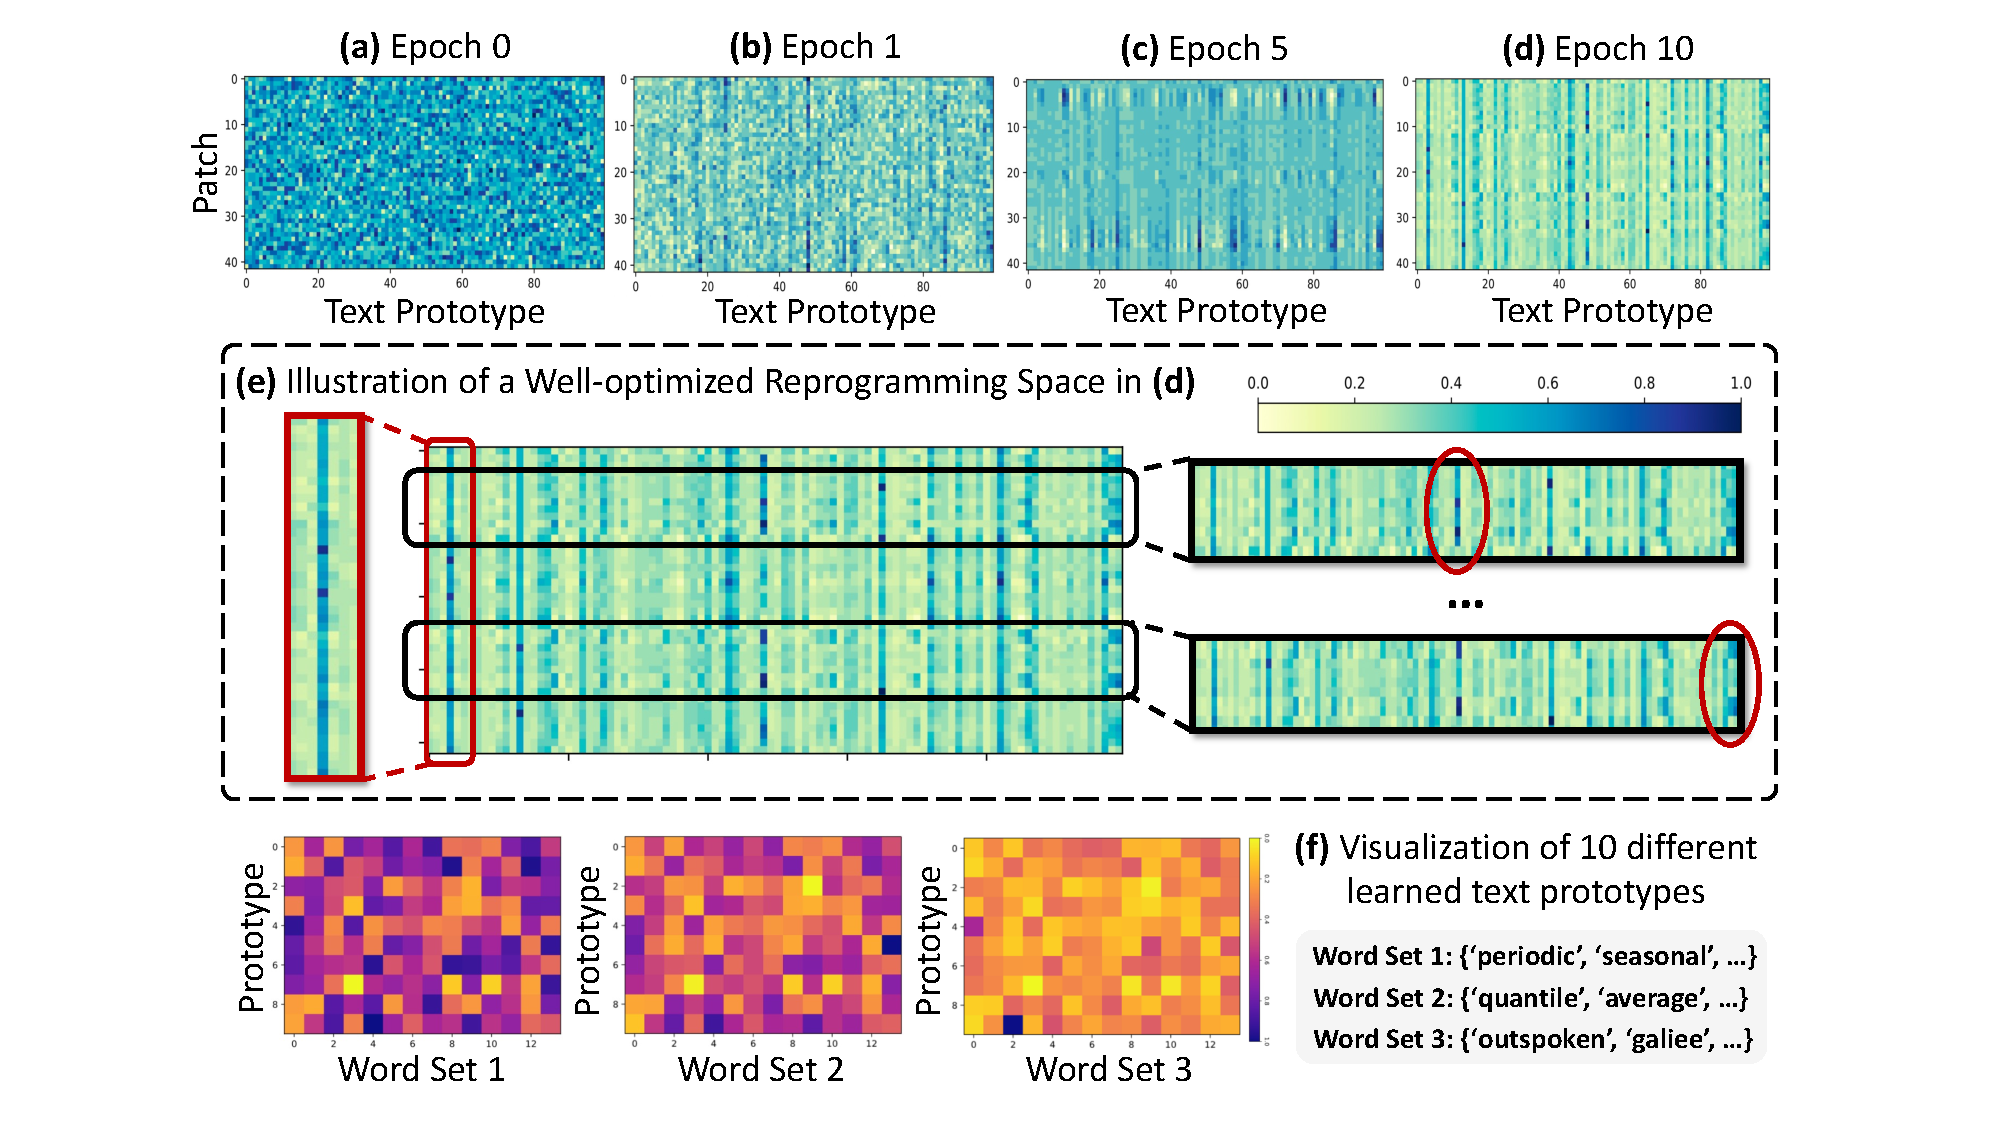
\includegraphics[width=7cm]{figures/reprogramming-showcase-v3.pdf}
\caption{A showcase of patch reprogramming.}
\label{fig:reprogramming_showcase}
\vspace{-4mm}
\end{wrapfigure}

\noindent\textbf{Reprogramming Interpretation.}
We provide a case study on ETTh1 of reprogramming 48 time series patches with 100 text prototypes in \shortautoref{fig:reprogramming_showcase}. The top 4 subplots visualize the optimization of reprogramming space from randomly-initialized \textbf{(a)} to well-optimized \textbf{(d)}. We find only a small set of prototypes (columns) participated in reprogramming the input patches (rows) in subplot \textbf{(e)}. Also, patches undergo different representations through varying combinations of prototypes. This indicates: (1) text prototypes learn to summarize language cues, and a select few are highly relevant for representing information in local time series patches, which we visualize by randomly selecting 10 in subplot \textbf{(f)}. Our results suggest a high relevance to the words that describe time series properties (i.e., word sets 1 and 2); (2) patches usually have different underlying semantics, necessitating different prototypes to represent.

\noindent\textbf{Reprogramming Efficiency.}
\shortautoref{tab:efficiency} provides an overall efficiency analysis of \method with and without the backbone LLM. Our proposed reprogramming network itself (\textbf{D.3}) is lightweight in activating the LLM's ability for time series forecasting (i.e., fewer than 6.6 million \textit{trainable} parameters; only around \textbf{0.2\%} of the total parameters in Llama-7B), and the overall efficiency of \method is actually capped by the leveraged backbones (e.g., \textbf{D.1} and \textbf{D.2}). This is favorable even compared to the parameter-efficient fine-tuning methods (e.g., QLoRA~\citep{dettmers2023qlora}) in balancing task performance and efficiency.

\begin{table}[t]
\captionsetup{font=small} 
\caption{Efficiency analysis of \method on ETTh1 in forecasting different steps ahead.}
\label{tab:efficiency}
\vspace{-4mm}
\begin{center}
\begin{small}
\scalebox{0.55}{
\setlength\tabcolsep{3pt}
\begin{tabular}{l|ccc|ccc|ccc|ccc}
\toprule

Length &\multicolumn{3}{c|}{ETTh1-96}&\multicolumn{3}{c|}{ETTh1-192}&\multicolumn{3}{c|}{ETTh1-336}&\multicolumn{3}{c}{ETTh1-512}\\

\midrule

Metric &Param. (M) & Mem. (MiB)  &Speed(s/iter) &Param. (M) &Mem. (MiB)  &Speed(s/iter) &Param. (M) &Mem. (MiB)  &Speed(s/iter) &Param. (M) &Mem.(MiB)  &Speed(s/iter)\\
\midrule

\textbf{D.1} LLama (32) &3404.53 &32136	&0.517	&3404.57  &33762	&0.582	&3404.62  &37988	&0.632	&3404.69 &39004	&0.697 \\

\textbf{D.2} LLama (8)	& 975.83 & 11370 &0.184	&975.87  &12392	&0.192	&975.92 &13188	&0.203	&976.11 &13616	&0.217 \\

\textbf{D.3} w/o LLM	& 6.39 & 3678	&0.046	&6.42 &3812	&0.087	&6.48 &3960	&0.093	&6.55 &4176	&0.129\\

\bottomrule
\end{tabular}
}
\end{small}
\end{center}
\vskip -0.2in
\end{table}
